\section{Couchbase}
Some of the general key properties of Couchbase, a document store database, are briefly outlined in the introduction. Later sections will take a closer look at specific characteristics and properties. The context of the CAP theorem will be addressed, as well as relevant characteristics and how they are realized in Couchbase Server. Overall this chapter will give the reader a closer understanding of the ideas behind Couchbase. A short paragraph on the history will provide some insight in the development of this NoSQL database. To cross reference the development steps with the increase of popularity of Couchbase, see \autoref{figure:Development} from this chapter’s introduction.\\
As a document store database Couchbase uses JSON documents to represent data as items \parencite{couchbaseAbout} \parencite{objelean}. As a common way to represent objects, especially in web development, the JSON format makes it easy to store and load data from a Couchbase database. The exact mechanics behind the data structures and the inclusion in buckets will be discussed as part of the core components in section \ref{section:corecomponents}.\\
Couchbase SDKs are available for most common programming languages (e.g. Java, .NET, Node.js, Python and more) and can be downloaded through the package management system of the respective development environment (e.g. Maven, Nuget, npm, pip and more) \parencite{couchbaseWeb} \parencite{objelean}. Thereby a widespread support is given. More information on SDKs and the usage follows in section \ref{section:SDK} of this chapter.
Other core characteristics of the Couchbase DB are: its memory-first architecture, an elastic scalability and an architecture based on buckets (which add redundancy and thereby persistence) \parencite{couchbaseWeb}. The core components as well as the architecture itself will be described more closely in the following sections.

\subsection{Couchbase History}
Couchbase DB is a NoSQL document store database that originated in the merge of Membase and CouchOne back in 2011 \parencite{couchbaseWeb}. Membase was build for applications that did not need SQL necessarily, but the durability, replication and data management that RDMS usually provide \parencite{ingenthron}. In the beginning the durability was achieved by MySQL in the background, storing memcached information on disk \parencite{popescuBacalu}. After the merge of CouchDB this responsibility was given to CouchDB implementation, resulting in a new product: Couchbase.\\
It started out as a “pure key-value database” \parencite{couchbaseAbout} till it 2012 became a JSON document-oriented database. 2015 SQL-like queries were introduced as well as multidimensional scaling \parencite{couchbaseAbout}. Ever since then, the database was adapted and extended, introducing features like Full-Text search (2017) and Analytics (2018) \parencite{couchbaseAbout}.

\subsection{Architecture}
Before looking at the core components of Couchbase let us take a quick overview of the basic concept behind the architecture of Couchbase and what makes it distinct from other databases.

\begin{figure}[H]
    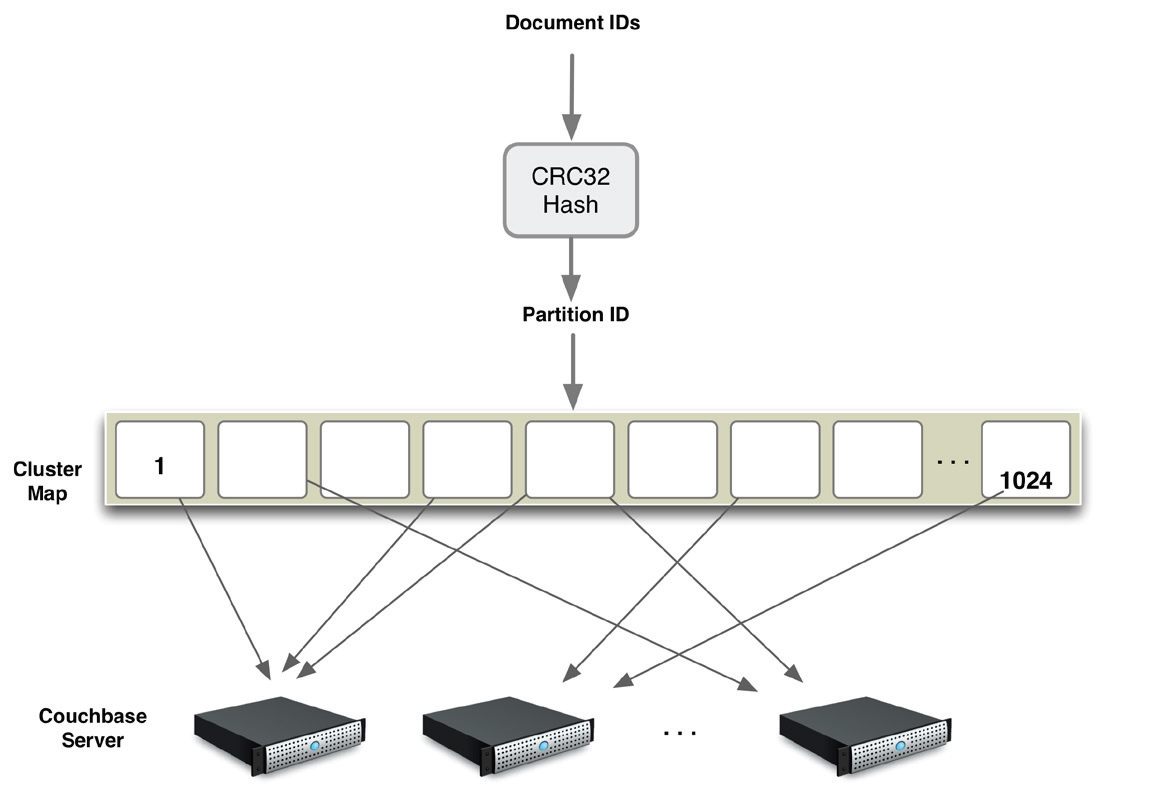
\includegraphics[width=\textwidth]{img/couchbaseClusterMap.jpg}
    \caption{Couchbase's sharding Architecture across its Cluster Nodes}
    \label{figure:Architecture}
\end{figure}

Couchbase was designed with a highly distributed architecture from the ground up, which makes it similar to other NoSQL databases. While it could be used on a single machine, the typical setting for Couchbase is a server cluster.
In this environment the data is stored by sharding it evenly across multiple machines. The system defines exactly 1024 partitions (not configurable) and (evenly) assigns them to the available nodes in the cluster. Once a document needs to be stored, the documentId - which is a unique identifier for every document - gets hashed to determine which of the partitions the data is assigned to. \autoref{figure:Architecture} illustrates this sharding process. Once the data is assigned, the document will be held in that partition. If nodes are added or removed from the cluster, Couchbase will reassign the partitions among all the nodes to rebalance itself. At any given time the nodes themselves are responsible for their assigned partitions. This leads to another property of Couchbase, which is that all the nodes are completely equal. Every node has two primary processes. The Data Manager is responsible for handling the actual data of the node's partitions while the Cluster Manager deals with the intra-node communication. Those are the reasons why Couchbase is excellent in scaling horizontally. \parencite{objelean}

To make sure that no data is lost when a node has a failure, a replication concept is necessary. Couchbase achieves this by replicating all the partitions and distributing them among the cluster, while making sure that the replica partition is never on the same physical server. This way, once a node fails the cluster will determine the location of the replica and make it the ‘active’ partition.

\subsection{Core Components}
\label{section:corecomponents}
This section will focus on some core components of CouchbaseDB. It will provide insight into the mechanics of the database and how the document based database concepts are implemented. To do so the low level concepts of buckets, data schemas and data limits are discussed. This will be the first step to understand availability, scaling and performance of a Couchbase Server infrastructure.
\subsubsection{Keys and Metadata}
The items, stored in documents, are made of keys and values \parencite{couchbaseDocuData}, where a key must be unique within the bucket. In case of nested objects (or attributes) the value can be regarded as an “embedded document” \parencite{couchbaseDocuData}, consisting of key-value pairs or further nested documents \parencite{couchbaseDocuData}. 
Along with the data itself metadata is stored by the server \parencite{couchbaseDocuData} \parencite{objelean} or in case of extended attributes possibly by the application \parencite{couchbaseDocuData}. The server metadata contains a unique ID, a revision or sequence number, an expiration time, flags and the document type\parencite{couchbaseDocuData}. The unique ID, also often simply called key, has the same purpose as the primary key in SQL. The revision or sequence number helps identify the number of mutations of a document, in case of update conflicts this helps find the newest or most current version of a document. The expiration time gives the document a time to live (TTL). This may be either set on document level or bucket level \parencite{couchbaseDocuMemory}. It uniquely identifies any document within the bucket. If the expiration times differ, the bucket TTL "wins" if the item TTL is longer. If it is shorter, the bucket TTL is left unchanged. Documents without a TTL are automatically given the bucket TTL if it is set \parencite{couchbaseDocuExpiration}. Flags and type metadata are used to identify the type of data as well as the type of the saved value. Extended attributes can either be system set or application set. Server internal extended metadata can “optionally be written and read by user applications” \parencite{couchbaseDocuData}, extended attributes set by the application however can only be accessed by the application which created it \parencite{couchbaseDocuExtendedAttributes}. All server internal metadata is kept in RAM, which leads to “100\% memory resident indexes” \parencite{couchbaseWeb} and provides extremely fast loading (performance).\\
There are some size limits for the documentId ("key"), the data ("values") and the metadata. The key size is limited to 250 bytes. The value plus the user extended attributes together can not extend 20 MiB. The system extended attributes have a maximum size of 1 MiB. Other fixed metadata such as the id, rev, expiration, flags and type have no limitation \parencite{couchbaseDocuData}.
\subsubsection{Document Store}
Documents in Couchbase DB are stored in JSON \parencite{objelean} or binary format \parencite{couchbaseDocuData}. Any document can be accessed using its unique key. JSON documents can further be parsed, indexed and queried. Binary format can only be retrieved by its key \parencite{couchbaseDocuData}. The general advantage of storing data in document form has already been discussed. In comparison to RDMS, object schemas used in an application can be applied directly as the schema for the document in the database.\\
This structure also “allows that data [can] be indexed and queried using views” \parencite{objelean}. Entries can be found using a JavaScript-based query engine which is provided by Couchbase Server. There are two main document design approaches to be considered. The first approach is storing a small number of rich documents. This leads to "fewer relations between independent objects" \parencite{couchbaseDocuDataModel} which in turn increases scalability. Also it is possible to group properties, typically accessed at the same time, increasing atomicity of operations. This is always a good idea since Couchbase guarantees that the ACID fundamentals are given for "all operations that address a single document" \parencite{couchbaseDocuDataModel}. The other design approach may be a large number of simple documents which possibly hold relations to each other. This is only feasible if the access-pattern is predictable and for some reason (e.g. network speed) the data-size has to be kept small. \\
The data model of Couchbase holds several advantages. For instance scalability is increased since replications and edits do not affect other documents other than the one replicated/ edited. There is no need to access or touch anything else in the database. Also the latency is kept low since no complex inter-node coordination has to be performed and all connections are minimized \parencite{couchbaseDocuDataModel}. The performance of Couchbase is further increased by the Sub Document API which lets the user access only parts of the inner components of a JSON document. The special Sub Doucment API can run a query against a specific path to either read or write (update) the attribute or document there \parencite{couchbaseDocuSubDoc}. The API was first introduced for Couchbase Server 4.5 and has been available all the way to the current version 6.0 \parencite{couchbaseDocuSubDoc}.
\subsubsection{Data Buckets}
To keep connected data records together, Couchbase Server implements buckets. Buckets are “isolated, virtual containers” \parencite{objelean}. On creation, they are assigned an innumerable name by which the bucket is accessed in the future \parencite{couchbaseDocuBuckMemStor}. No item can be saved before a bucket exists for it \parencite{couchbaseDocuMemory}. Buckets can be replicated leading to redundancy and failure copies \parencite{couchbaseWeb}. There are three types of buckets provided, differing in their way of storing data: Couchbase buckets, Ephemeral buckets and Memcached buckets \parencite{couchbaseDocuMemory}.\\ 
Couchbase Buckets store data both persistently on disk and in memory. High availability is given since data is automatically replicated using the Database Change Protocol (DCP) and scalability accomplished through Cross Data Center Replication (XDCR) "dynamically scaled across multiple clusters" \parencite{couchbaseDocuBuckets}. If the memory capacity to store data there runs out there are two strategies to eject items from memory. Either value-only, meaning only the value is ejected and the key and metadata kept in RAM, or a full removal strategy. Value-only provides less freed room in memory but will keep up good performance since data can easily be accessed on disk by its unique key. A full removal will lead to more freed memory but less performance since the disk needs to be queried for every request \parencite{couchbaseDocuBuckets}.\\
Ephemeral buckets are used when persistence is not required. Data is only kept in memory, leading to a highly-consistent in-memory performance. This can be seen especially in case of a rebalance (when a node is added or removed and the system needs to redistribute) and on restart \parencite{couchbaseDocuBuckets}. If this bucket runs out of available memory there are again two strategies: Either it is generally forbidden to add more data than there is room available, which leads to a fail or data is ejected, which leads to a data loss since no data is saved persistently on disk \parencite{couchbaseDocuBuckets}. \\
Memcached Buckets cache frequently used data and thereby reduce the number of queries. They provide a directly addressable, distributed, in memory key-value cache \parencite{couchbaseDocuBuckets}. As in-memory suggests, no data is stored on any disk, everything is kept in RAM. If the RAM quota is exceeded data will be ejected and lost.\\
Couchbase and Ephemeral Buckets are the most commonly used, they "both provide a highly available, dynamically reconfigurable, distributed data-store" \parencite{couchbaseDocuBuckets}. Persistence for Couchbase Buckets is achieved asychronously between memory and disk. Ephemeral Buckets are only persistent in RAM. Replication, using both DCP and XDCR, is both in Couchbase Buckets and Ephemeral Buckets configurable over a number of servers. For Couchbase Buckets a host server failure leads to the promotion of the replica server which guarantees high availability. For Ephemeral Buckets, the ones which eject data are not permitted to do XDCR though they can be the target of XDCR operations \parencite{couchbaseDocuBuckets}. Rebalance is handled in the same way for Couchbase and Ephemeral Buckets. As buckets and nodes are dynamically added or removed, the buckets and data are distributed evenly across all available nodes \parencite{couchbaseDocuBuckets}.\\
To increase performance further there are three modes of compression available for Couchbase Sever and data passed through it. This leads to more efficient RAM and disk space usage, reduced need of network bandwidth and higher consumption of CPU \parencite{couchbaseDocuCompression}. Compression is provided by the open-source library "Sappy" and is works specific to the clients capabilities. The compression mode can be established by the user per bucket \parencite{couchbaseDocuCompression}. The available modes are: off, passive and active.\\
Off is recommend for clients which will not benefit from compression and if bandwidth usage is no issue. If data is received compressed it will be decompressed to be stored in memory and recompressed to be stored on disk. It is always returned in uncompressed form. Memcached buckets only operate on this mode\parencite{couchbaseDocuCompression}. \\
the passive mode stores data compressed both in memory and on disk. Data is returned uncompressed unless requested otherwise. Then, data can be returned compressed as well. It is the job of the client to know if it can process compressed data and request accordingly. If uncompressed data is received however, it will only be compressed for disk storage, not in memory. It is then returned uncompressed as well. Advantage of this mode are the reduced memory usage and bandwidth and the reduced CPU usage for the clients that do not required a compressed format \parencite{couchbaseDocuCompression}.\\
Active mode stores data compressed in memory and on disk no matter what the client handed in. If a client does not support receiving compressed format, it is decompressed before sending it out. This maximizes memory space and network usage. At the cost of wasting CPU time on compression for a client that will need decompressed data as return data \parencite{couchbaseDocuCompression}.
\subsubsection{VBuckets}
vBuckets, sometimes called “shards”, are “defined as owner of a subset of the key space of a Couchbase cluster” \parencite{objelean} \parencite{couchbaseDocuVbuckets}. They are used to implement both Couchbase and Ephermal buckets \parencite{couchbaseDocuVbuckets} and have organizational functions such as the distribution of data and replication on more than one node \parencite{objelean} \parencite{couchbaseDocuVbuckets}. Replications are distributed across the cluster. Write operations can only be performed on active buckets, read requests are mostly performed on the active vBucket \parencite{couchbaseDocuVbuckets}. Per bucket, 1024 vBuckets (or 64 on MacOS) are created \parencite{couchbaseDocuVbuckets}. In case of a replication of said bucket all 1024 (or 64) vBuckets are copied \parencite{couchbaseDocuVbuckets}, leading to 2048 vBuckets stored.  Data items are stored evenly across all vBuckets. \\
To locate and access an item the document key is consulted. The documents all have unique identifiers (the key), which are associated with a specific vBucket using a hashing function mapping \parencite{objelean} (a CRC32 hashing algorithm \parencite{couchbaseDocuVbuckets}). Using this algorithm and the id, the bucket number can be calculated. This number is used to to find the server that “hosts” the vBucket using a map to determine the correct server node \parencite{couchbaseDocuVbuckets}. The mapping of vBucket to individual node is handled by the Cluster Manager \parencite{couchbaseDocuVbuckets}. After the node has been identified the operation can be performed directly on this server node. \\
In case of a cluster-configuration change (addition or removal of nodes) first the replica buckets are promoted if applicable. It is applicable in case the active buckets are lost due to a failure or deletion. After that, primary and replica buckets are redistributed across the newly available buckets. Last the Cluster Manager updates the mapping and sends it out to all cluster-partitions \parencite{couchbaseDocuVbuckets}.

\subsection{Querying}
\subsubsection{N1QL} \label{n1ql}
Couchbase has its own query language called N1QL (pronounced "nickel") \parencite{couchbaseDocN1Ql}. Even though Couchbase Server is a NoSQL database, N1QL is very similar to SQL in syntax and use. However, as the information can be nested within documents N1QL features some additions that are not needed in SQL. The basic clauses in N1QL are: 
\begin{itemize}
    \item SELECT
    \item FROM
    \item LET
    \item WHERE
    \item GROUP BY
    \item ORDER BY
    \item LIMIT
    \item OFFSET
\end{itemize}
The expression used in a SELECT statement can be either literal values, calculations or properties from documents. If the properties are specified in the statement, the result will contain only the given properties from matching documents. It is possible to use a wildcard selector (*), in which case the query returns each matching document in its entirety. The id that is assigned to each document by Couchbase Server is not included when retrieving the complete document. To get this information, the META() function needs to be utilized. It returns a document that contains metadata about the document it belongs to. Its properties like the documentId can be accessed via a "dot" notation: META().id \parencite{proCouchbaseServer}.\\
The FROM statement is where the source to retrieve data from is defined. In SQL this is the name of the database. Similarly, in N1QL the name of the bucket to search in is given. However, this is not the only type of source that can be stated. It is possible to query only from certain properties (or even properties of properties) if necessary. Again, this utilizes the simple "dot" notation  \parencite{proCouchbaseServer}. An example of this would be: \texttt{SELECT * FROM userdata.user.role}. This query retrieves all properties from the role property of the user property from documents in the userdata bucket. This allows developers to build more flexible queries when dealing with heavily nested structures. Another option to define the source is to use a subquery. This means that within the FROM clause, another query is being executed, the result of which is used as the source for the outer query \parencite{couchbaseDocN1Ql}. Just like in SQL, N1QL allows for joins of different sources. The JOIN ... ON KEYS clause, which is used to execute joins, takes a property from one bucket which is then used as a key in another bucket. For example \texttt{SELECT * FROM books AS b JOIN authors AS a ON KEYS b.author;} returns all documents from the "books" bucket with additional info from the "authors" bucket, looked up in authors with author property in books. \\
The LET statement makes it possible to define variables to use in other parts of the query. The value of a variable can be the result of a subquery. The WHERE clause allows for filtering of documents for specific characteristics. In it, developers can execute calculations and create boolean expressions by comparing values or combining boolean values with AND or OR clauses \parencite{couchbaseDocN1Ql}. To group resulting documents together, the GROUP BY clause is used. Given a property, it aggregates certain values according to the property. The ORDER BY clause orders the results by a given property \parencite{proCouchbaseServer}. To reduce the number of documents shown in the result, a maximum number can be set using the LIMIT clause. The given number corresponds to the amount of result documents. The OFFSET clause is used to not start with the first document, but with a later one. If the Limit is 1 and the Offset is 1 as well, only the second document from the entire result will be returned \parencite{proCouchbaseDev}.
\subsubsection{Views}
Couchbase offers another way to retrieve data: views. They allow developers to create more complex queries by writing their own functions and perform calculations on the data in the same step. Views use the MapReduce programming model to enable them to process documents across a cluster. For each view a map function is defined, which is applied to every document in the bucket and takes care of the initial filtering and processing of the documents \parencite{proCouchbaseServer}. The result of the map function is an index, which is a list of key-value pairs. This index is then stored on the disk and is updated when the documents change \parencite{couchbaseDocViews}. Each view can also have a reduce function, which performs aggregations on the data. Couchbase Server provides commonly used reduce functions (e.g. basic statistical functions) \parencite{proCouchbaseServer}. Once the map and reduce functions are defined, the view can be queried. Every time a view is queried, Couchbase Server builds a new index by default, to make sure that all changes that were made since the last query are in the index. As building an index takes up a lot of resources, developers can decide depending on their application wether or not a new index should be built for every view queried \parencite{couchbaseDocViews}.


\subsection{Performance}
When deciding which database to use for an application, it is important to consider its performance under high load. The instantiation of a Couchbase bucket is faster than of an SQL database, but slower than other NoSQL databases. When tasked with executing a large number of reading operations, Couchbase proves to be more efficient than other databases, handling even large amounts of operations very fast. The same result applies to delete operations \parencite{compNoSQLandSQL}.  As for loading data into the database, Tang and Fan (\parencite{insert}) showed that Couchbase performed inserts faster than Cassandra and HBase, but slightly slower than Redis and MongoDB. Additionally, they state that the performance decreases in comparison to other NoSQL databases with an increasing number of documents to be inserted.


\subsection{Monitoring}
To setup and maintain your Couchbase database, the Couchbase Web Administration Console offers a lot of information and direct interaction with your database. Part of that is the monitoring section, which provides details on resources used by the cluster, each node or bucket. The level of detail one wishes to see is adjustable. Additionally, the Web Administration Console not only shows numbers, but visualizes them as graphs so they are easier to grasp \parencite{getStarted}. The overview of the entire cluster shows information on resource usage across buckets, e.g. RAM available for the cluster, RAM used by buckets and RAM allocated by buckets. Similar information is given for the disk space that is used. In addition, graphs provide insight about the operations and disk fetches per second, which are valuable to keep an eye on the overall condition of the database and the application it is used for. \parencite{proCouchbaseServer}.

\begin{figure}
    \centering
    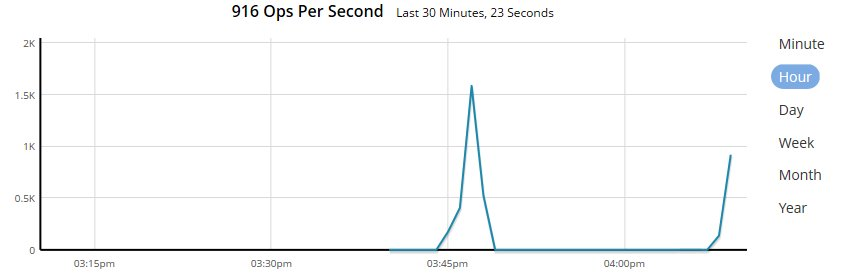
\includegraphics[width=\textwidth]{img/couchbaseMonitorOps.jpg}
    \caption{Monitoring the operations per second}
    \label{figure:ops}
\end{figure}

\autoref{figure:ops} shows two spikes in operations per second in the last hour, which timestamps correspond to the queries executed before.

\begin{figure}[H]
    \centering
    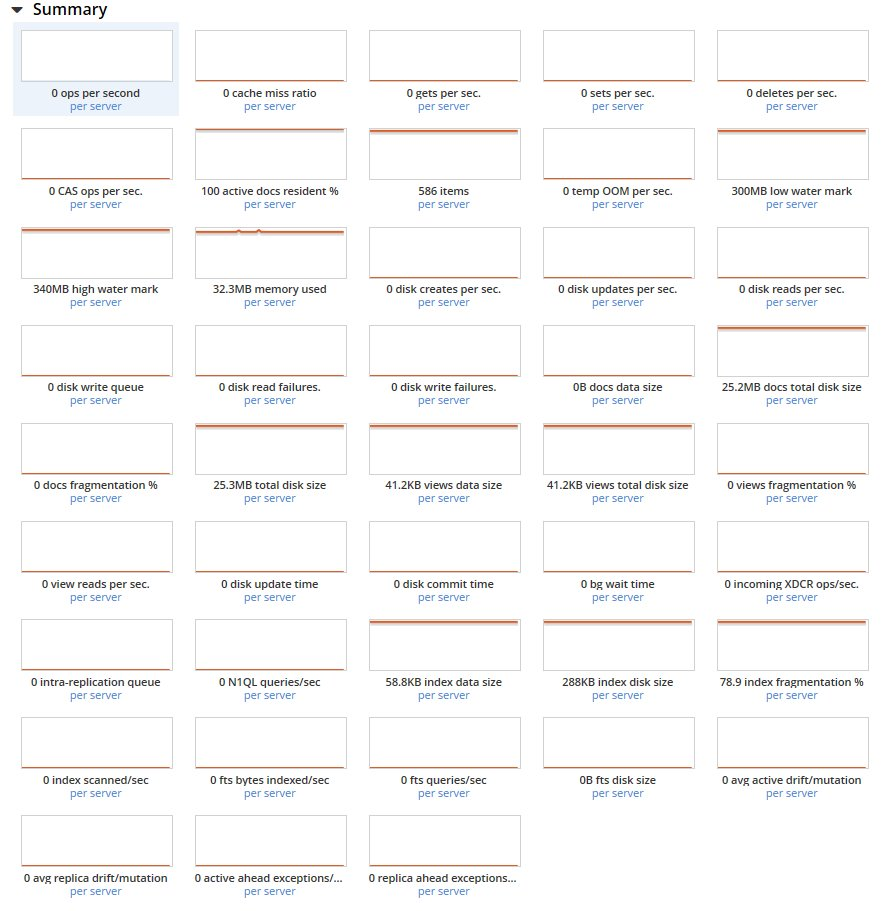
\includegraphics[width=\textwidth]{img/couchbaseMonitor.jpg}
    \caption{Monitoring metrics of an individual bucket in Couchbase}
    \label{figure:Monitoring}
\end{figure}

\autoref{figure:Monitoring} shows all the graphs available for individual buckets. All in all, over forty metrics can be viewed and used to assess the health and performance of the system.

\subsection{CAP Theorem}
From a CAP-Theorem perspective Couchbase can be operated as a CP or CA system. By default it will act as CP system. When a Node fails some data will be temporarily unavailable for writes until the replica is set to active. However, reads will be processed regularly by the replicas available in the cluster. If needed, it can be tuned to act as a CA system for example through auto-failover. But this is only half the story and only applies if Couchbase is run in a single cluster setting. With a multiple cluster setting, also known as Cross Data Center Replication (XDCR), it will act as AP system. Since in this setting any Cluster can be written to, problems arise when the same data is modified from different locations. In this case Couchbase provides different configurations for conflict resolution (for example through timestamp or revision ID), eventually leading to consistency between multiple clusters. \parencite{couchbaseCAP}

\subsection{SDK}
\label{section:SDK}
To use Couchbase productively in a development environment this last section shall discuss the available software development kit and give some examples on how to use it to perform basic CRUD operations on the cluster's data.\\
First of all, Couchbase offers SDKs for several popular programming languages and runtime environments inlcuding C, Go, Java, .NET, Node.js, PHP and Python. \parencite{couchbaseSDK} Since it would be out of scope to give examples for all of them, this section will limit the examples to the Node.js SDK, but the information given will be easily transferable to other languages as well.

First, a connection to the Couchbase Cluster needs to be established. Afterwards, authentication is necessary to select the desired bucket. Once there is a bucket object it can be used to send queries. The described steps can be seen in Listing \ref{couchbaseAuthAndBucket}.\\
\begin{listing}[ht]
\begin{minted}{js}
const cluster = new couchbase.Cluster('localhost:8091');
cluster.authenticate('user', 'password');
const bucket = cluster.openBucket('demo-bucket');
\end{minted}
\caption{Connect to Couchbase}
\label{couchbaseAuthAndBucket}
\end{listing}

\newpage
Two different kinds of interacting with the data shall be looked at. The first option is to use the core operations upsert(docId, document), insert(docId, document), replace(docId, document), get(docId) and remove(docId) to execute the basic CRUD operations. Insert will only insert the document if the docId isn't found, replace will only replace the document if the docId is found and upsert will always replace the document (ignoring if the docId existed or not). The second option is to use N1QL queries described in \autoref{n1ql} to query the desired data. Examples for both options can be seen in Listing \ref{couchbaseCRUD} and Listing \ref{couchbaseSDKN1QL}.\\

\begin{listing}[ht]
\begin{minted}{js}
// Remove and Get use the same syntax
bucket.get('uniqueDocId', function(err, res) {
    if (err) {
        console.log('operation failed', err);
        return;
    }
    
    //res contains the document
    console.log('success!', res);
});

// Replace, Insert and Upsert use the same syntax
bucket.insert('unqiueDocId', {some:'value'}, function(err, res) {
    if (err) {
        console.log('operation failed', err);
        return;
    }

    console.log('success!', res);
});
\end{minted}
\caption{CRUD Operations}
\label{couchbaseCRUD}
\end{listing}

\begin{listing}[ht]
\begin{minted}{js}
const q = couchbase.N1qlQuery.fromString('SELECT airportname as n
    FROM `travel-sample` where type="airport" LIMIT 4');
// Using arrow functions to iterate through the result set
bucket.query(q, (err, rows) => rows.forEach((row) => console.log(row)));
\end{minted}
\caption{Query Data with N1QL}
\label{couchbaseSDKN1QL}
\end{listing}
\newpage
It is important to note that while in earlier versions of the SDK it was not possible to stream the results of N1QL queries row by row (and instead had to wait for the complete result set) recent versions do not have this limitation anymore.

It should be clear that the presented examples are far from showing all of the offered capabilties of the Couchbase SDK and merely offer an easy introduction. To explore more of its capabilities, like MapReduce Views or Concurrent Document Mutations, the Couchbase Documentation is an excellent place to start.

\subsection{Conclusion}
To sum it all up there are several key takeaways from this research into Couchbase, its mechanics and its take on the CAP theorem. High performance in Couchbase is achieved due to the partitioning into small vBuckets, compressed data transmission and in memory strategies for at least the most important metadata (unique documentId). In terms of the CAP-Theorem the decision whether Couchbase is rather AP (Availability and Partition Tolerance) or CP (Consistency and Partition Tolerance) depends strongly on the cluster setup. What can be said, especially in comparison to relational databases, is that Couchbase (same as most document oriented databases) scales well horizontally. A reason for that is the vBucket partitioning and the equality of nodes.

Use Cases that make Couchbase a good database choice are cases of large amounts of unstructured data. Due to the not fixed schema, Couchbase can work with changing requirements of application object structure or general data schema. Another scenario where Couchbase stands out against other document oriented databases are performance scenarios.

This chapter gave you a broad overview of Couchbase, its components and its classification within the CAP theorem. Other very important aspects of modern databases could not be covered however. The aspects security and user permission management were not discussed and are to be researched further in the future.